%\documentclass[10pt,journal,compsoc]{IEEEtran}
\documentclass{vldb}
\usepackage{graphicx}
\usepackage{balance}  % for  \balance command ON LAST PAGE  (only there!)
\usepackage{placeins}
\usepackage{array}
\usepackage{graphicx}
\usepackage[usenames, dvipsnames]{color}

\makeatletter
\def\@copyrightspace{\relax}
\makeatother

\begin{document}

% ****************** TITLE ****************************************

\title{The \textcolor{red}{WAK} Audio Codec: Stereo and Huffman Coding}
\subtitle{Stanford University \\ Center for Computer Research in Music and Acoustics \\ (wisam,ameacham,kaichieh)@ccrma.stanford.edu}

% ****************** AUTHORS **************************************

\numberofauthors{3} 
\author{
% 1st author
\alignauthor
\textcolor{red}{W}isam Reid\\  
% 2nd. author
\alignauthor
\textcolor{red}{A}idan Meacham\\
% 3rd. author
\alignauthor
\textcolor{red}{K}ai-Chieh Huang\\
}
\maketitle

% \begin{abstract}
% Abstract goes here.
% \end{abstract}

\section{Project Overview}
The WAK coder operates on the principle of redistributing coding gains during ``easy'' parts of a track to more difficult sections as a result of its primary components, Huffman coding and joint stereo coding. Each of these processes realizes a coding gain over the baseline single channel coder by identifying further redundancies (between mantissa symbol representations and stereo channel correlation, respectively) and modifying the bit allocation routines. The data savings are then passed on to later blocks that may need additional overhead to achieve total masking of the quantization noise. Our goal is to achieve high signal quality at 128 kbps per channel, and for many signals, we achieved the specification. The main building blocks of our stereo codec is presented in  \textbf{Fig~\ref{fig:encoder}} and \textbf{Fig~\ref{fig:decoder}}.

% ENCODER FIGURE
\begin{figure}[h] 
\centering
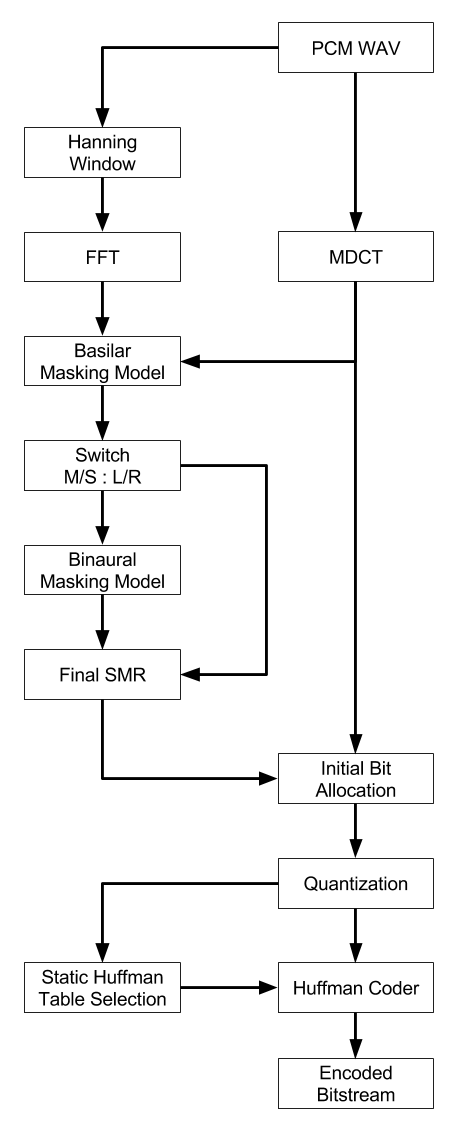
\includegraphics[height=3 in]{PAC_Encoder_Block_Diagram}
\caption{Encoder Diagram}
\label{fig:encoder}
\end{figure}

\section{Huffman Coding}
Huffman coding is an entropy encoding algorithm \cite{Huffman1952} used for lossless data compression and is commonly used in media compression such as video and audio. By using Huffman coding, we can efficiently allocate bits to represent symbols in the data by exploiting the probability of their occurrence, where symbols with high occurrence being assigned fewer bits than less common symbols. 
As a result, the compression ratio of Huffman coding increases as the unbalanced degree of symbol probabilities. Since the Huffman code depends on the probabilities of each symbol, it can give coding gain when there are strong temporal correlations between consecutive amplitude values. Furthermore, Huffman coding provides lossless compression by recovering the original symbol representation from the Huffman table used to compress, hence maintaining the output quality of the coder. In audio compression scene, Huffman coding can be used to further encode quantized mantissa bits to lower the data rate or improve the sound quality at a fixed data rate by reallocating bit savings from Huffman coding back into the next block's mantissas. 

% DECODER FIGURE
\begin{figure}[h] 
\centering
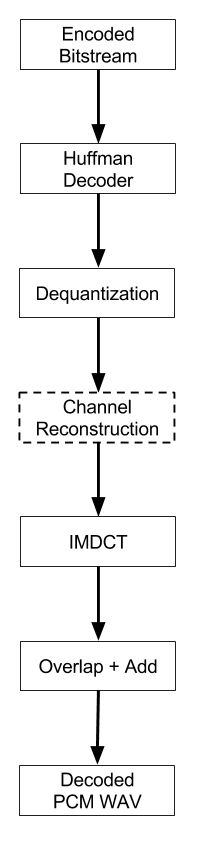
\includegraphics[height=3 in]{PAC_Decoder_Block_Diagram}
\caption{Decoder Diagram}
\label{fig:decoder}
\end{figure}

\subsection{Description}
In general, Huffman coding can be categorized into two genres: dynamic table and static table Huffman coding. In dynamic table Huffman coding, a Huffman table is generated from the original data and passed along with the compressed file. While decoding, the decoder extracts the Huffman table from the compressed file and uses it to recover the original data. Because the Huffman table is generated dynamically at the encoding stage based on the data to be compressed and passed along to the decoder, this genre of Huffman coding is guaranteed to work on any data passing in, and therefore is more straightforward and easier to implement. However, the Huffman table concealed in the compressed file can lower the compression ratio depend on its size. 

On the other hand, static table Huffman coding provides higher compression ratios by excluding the Huffman table from the compressed file and uses a list of pre-constructed tables to encode and decode data. Since the performance of Huffman coding is related to the symbol probability distribution, the compression ratio of static Huffman coding can be lower than dynamic Huffman coding if there's no suitable match in the list of pre-constructed tables. Thus, in order to maintain a robust compression ratio, a wide range of sample data is required in the training stage to construct a sufficient number of tables.

It is worth noticing that some of the symbols may not be present in the pre-constructed tables when encoding data that was not used for training. Hence, an escape code is typically used to address this issue by using this special code to inform the decoder which part of the code in the bit stream is not Huffman encoded. 

In general, static Huffman coding is used for audio codecs due to the constraint on bit budget. Moreover, the audio quality of the audio codec at a fixed bit rate is considered to be the most important issue. By using static Huffman coding, we can have higher bit savings to reallocate than  dynamic Huffman coding, resulting in better sound quality. We will discuss a more detailed implementation in the following sections.

\subsection{Implementation Detail}
Considering the fact that there is plenty of literature on Huffman coding, we will only briefly introduce the general idea of constructing the Huffman code and focus more on the implementation detail of integrating static Huffman coding into our audio codec. To construct the Huffman table, we first count the occurrence frequency of each mantissa code we encountered in the audio data and use this knowledge to build a Huffman tree.

The Huffman tree is generated by creating a Huffman node for each mantissa code, with its occurrence frequency stored in the Huffman node. Then, we join two nodes at a time from the lowest occurrence frequencies and view them as one node with the sum of their occurrence frequencies. After joining all of the nodes, we will eventually be left with only one Huffman node that is denoted as the root of the Huffman tree. By traversing down the Huffman tree and assign a 0 bit while traversing left and a 1 bit otherwise gives the Huffman code for each mantissa code at the leaf nodes. In the decoding stage, the decoder reads 1 bit at a time in the bit stream until there's a corresponding Huffman code in the static Huffman table used to encode the particular block.

Since the first bit of mantissa code in block floating point quantization is the sign bit and it occurs almost fifty percent on each sign due to the nature of audio signal, including the sign bit while constructing the Huffman table will only make our table larger without affecting the performance much. In our implementation, we strip off the sign bit of each mantissa code before Huffman encoding and code the sign bit before all the Huffman codes in each scale factor band. Note that since we only encode the mantissa code without the sign bit, we also need to construct the static Huffman table based on counting the unsigned mantissa codes in the training stage.   

After building the static Huffman tables through the training stage, we can now Huffman encode and decode the mantissa codes by passing only the table ID to the decoder to inform which static Huffman table was used to encode the mantissa codes. In this project, our audio codec runs Huffman coding on a per-block basis. For instance, while encoding each block, we test all possible tables before selecting the table that produces the shortest Huffman encoded mantissas for this block. Four bits in each block are used to inform the decoder which table ID to use for decoding at the beginning of each block. This way, the encoder can automatically select the table that gives the best result and encodes the data using that table. The detail on generating the static Huffman tables for our WAK audio codec is presented in the next section.

\subsection{Table Pre-construction}
In this project, we generated ten static Huffman tables during the training stage. The ten tables are trained with ten audio sound genres including rock, pop, speech, percussion, piano, traffic noise, gunfire, classical music, jazz, and rich harmonic (tonal structure) sounds such as guitar and harpsichord. The six most common symbols (mantissa code) presented in each table and their corresponding Huffman code is presented in \textbf{Table~\ref{table:huffmancodes1}}, \textbf{Table~\ref{table:huffmancodes2}}, and \textbf{Table~\ref{table:huffmancodes3}}.

While counting the frequency of occurrence for each symbol, we counted the occurrences of each mantissa integer value. Since the maximum mantissa bits in the codec is set to be 12 bits, we will assume the mantissa integer value is a 12 bit mantissa code as presented in the tables. The table for piano, speech, percussion, pop and tonal structure are trained using seven, five, six, four and six sound files respectively. Since we later found that the result of using multiple sound files gave us little advantage compared to using only one sound file, the rest of the tables are trained using only one sound file to represent the particular genre.

\begin{table}[h]
  \centering
    \begin{tabular}{ | l | l | l | l | l |}
      \hline
      Mantissa code & Piano & Speech & Percussion & Pop \\
      \hline
      000000000000     & 1      & 1      & 1       & 1   \\
      000000000001     & 011      & 011      & 011     & 011  \\
      000000000010     & 0100      & 000     & 000      & 000 \\
      000000000011     & 01011      & 0011     & 0011    & 0011  \\
      000000000100     & 00110      & 01010     & 01010     & 01010  \\
      000000000101     & 00001      & 00100     & 00100     & 00100  \\
      \hline
    \end{tabular}
  \caption{Six most common mantissa codes for static Huffman tables -- Piano, Speech, Percussion, and Pop}
  \label{table:huffmancodes1}
\end{table}
\begin{table}[ht]
  \centering
    \begin{tabular}{ | l | l | l | l | l |}
      \hline
      Mantissa code & Tonal & Jazz & Gunfire & Rock \\
      \hline
      000000000000     & 1      & 1      & 10       & 1   \\
      000000000001     & 00      & 01      & 1111     & 01  \\
      000000000010     & 0111      & 000     & 11100      & 000 \\
      000000000011     & 01101      & 00111     & 111010     & 00111  \\
      000000000100     & 01011      & 00100     & 11011110     & 00101  \\
      000000000101     & 011001      & 001011     & 111011100     & 001100  \\
      \hline
    \end{tabular}
  \caption{Six most common mantissa codes for static Huffman tables -- Tonal, Jazz, Gunfire, and Rock}
  \label{table:huffmancodes2}
\end{table}
\begin{table}[ht]
  \centering
    \begin{tabular}{ | l | l | l | }
      \hline
      Mantissa code & Traffic & Classic \\
      \hline
      000000000000     & 1      & 111       \\
      000000000001     & 00      & 110111       \\
      000000000010     & 0110      & 110011     \\
      000000000011     & 01111      & 11011000    \\
      000000000100     & 01010      & 11011010      \\
      000000000101     & 011101      & 110110110     \\
      \hline
    \end{tabular}
  \caption{Six most common mantissa codes for static Huffman tables -- Traffic and Classical Music}
  \label{table:huffmancodes3}
\end{table}

\subsection{Escape Codes}
As mentioned previously, an escape code is necessary for each static Huffman table to resolve the issue of unexpected symbols from the actual data to be compressed. Since we do not have a Huffman code for the unforeseen mantissa codes, we can only partially Huffman encode the audio file. Nevertheless, the decoder has no information on which part of the bit stream is Huffman encoded or not. We thus need to use an escape code to inform the decoder which sections of the bit stream contains original mantissa codes.

While Huffman encoding, a mantissa code that is not present in the static Huffman table is encoded as the escape code followed by the original mantissa code. At the decoding stage, when the decoder discovers an escape code, it uses the bit allocation information (how many bits were used by the original mantissa code) to read in the original mantissa code followed by the escape code. When generating the static Huffman table, all mantissa codes that appear infrequently are grouped into one category that accounts for the probability of a rare symbol occurrence while encoding an audio file.

While traversing the Huffman tree to construct the Huffman code for each mantissa, a Huffman code will be assigned to this rare symbol group and serve as the escape code described above. For our implementation, we discard all the mantissa codes with less than ten occurrences and group them into the rare mantissa category. In \textbf{Table~\ref{table:huffmanescape}} we show the escape codes used in each of the ten static Huffman tables for our WAK audio codec.

\begin{table}[ht]
  \centering
    \begin{tabular}{ | l | l | }
      \hline
      Tables & Escape Code  \\
      \hline
      Piano     & 0010100     \\
      Speech     & 0101110    \\
      Percussion   & 0100111 \\   
      Pop     & 011000100 \\    
      Tonal     & 01000101 \\     
      Jazz     & 001010110\\ 
      Gunfire & 111011000100 \\
      Rock    & 00100101001 \\
      Traffic  & 0101111 \\
      Classic  & 1101101111110 \\
      \hline
    \end{tabular}
  \caption{Escape codes for each static Huffman table in the WAK audio codec}
  \label{table:huffmanescape}
\end{table}

\subsection{Relationship with VBR Pool}
By using Huffman coding to further compress the audio data, the bit savings from this statistical compression of mantissas is placed into a variable bit rate pool that is shared from block to block. The next time the bit allocation routine is run, it will have a larger budget to reduce the quantization noise. It is worth noticing that the static table Huffman coding used in the audio codec saves bits by lowering the average bits used in each block. Thus, it is possible that some blocks will need more bits after Huffman encoding. This is essentially similar to borrowing bits from future blocks, and hence has potential to exceed the bit budget if we were to reallocate the bits saved by Huffman encoding directly to the next block.

The most secure way is to count the net bits savings after Huffman encoding the whole audio file then reallocate bits to the MDCT bin that has the highest quantization noise. This approach is very inefficient and cannot be implemented in real time, since we would need to go over the audio file more than once. A naive but efficient solution is to only allocate a lower percentage of bit savings from block to block after Huffman encoding to stay below the bit budget. The number of percentage chosen is based on empirical testing on the audio codec and an understanding of the average bit savings made by Huffman coding. 

\subsection{Results}
After implementing the Huffman coding for our audio codec, we tested it on six genres that are commonly seen. Furthermore, the audio files tested are all not presented in the training stage while constructing static Huffman tables. The six genres we tested are piano, speech, percussion, pop songs, highly tonal samples, and rock songs. The compression ratio for each genre tested is derived by averaging the result of 3 audio files. For pop songs and rock songs, each file is approximately 20 seconds, and other genres' file length is around 10 seconds.

An overview on the resulting compression ratio improvement comparing to the original 128/kb per channel baseline codec for each genre is presented in \textbf{Table~\ref{table:huffmancompression}}. As we can see from the table, there the performance of the Huffman coding varies between genres. This result is related to the static Huffman table we trained before using the audio codec to encode general audio files. Nevertheless, an average of 8.05 \% compression ratio is improved after Huffman coding the mantissas compare to our baseline codec. These bit savings from Huffman encoding can provide extra bits to some block with higher quantization noise to improve the quality of the audio file at a similar data rate before Huffman coding.

As discussed in the previous section, we implemented the bit reallocation in our WAK audio codec as giving a certain percentage of the bit savings from Huffman coding to the next block and traverse one pass through the audio file. The result of reallocating 1\% of bit savings from Huffman coding is also presented and compared in \textbf{Table~\ref{table:huffmancompression}}. The number 1\% is chosen based on empirical testing as described above.

\begin{table}[ht]
  \centering
    \begin{tabular}{ | l | l | l |}
      \hline
      Genre & Without Bit reallocation & Bit reallocation \\
      \hline
      Piano     & 5.60 \%   & 1.88 \%  \\ 
      Speech     & 3.91 \%  & 2.00 \% \\
      Percussion   & 13.56 \% & 3.33\% \\   
      Pop     & 11.84 \% &  1.55 \%\\    
      Tonal     & 3.72 \% &  3.37 \%\\     
      Rock     & 9.75 \% &  1.80 \%\\ 
      \hline
    \end{tabular}
  \caption{Compression ratio for Huffman encoding, with and without bit reallocation}
  \label{table:huffmancompression}
\end{table}

\section{Stereo Coding}
One may consider how to exploit redundancy between two highly-correlated channels to reduce the throughput required for reproduction, especially since audio is most commonly presented in stereo. Generally speaking, if the left and right channels of a stream share similar tonal content, then the difference between the two is low by definition. In the degenerate case, where two identical mono streams are transmitted, it is obvious that subtracting the channels block by block would result in a zero output. This can be exploited by virtue of the low bit allocation needed to adequately represent this small signal.

Because of the nature of this decomposition, the method is often referred to as ``sum and difference'' or ``middle / side'' encoding. The decomposition and reconstruction process is lossless without quantization, and is therefore a good fit for high-quality audio coding.

\subsection{Description}
We developed two versions of the WAK coder which differ primarily in how they pick whether a given band will be coded with the LR channels or the MS channels. We will discuss the second version below with respect to bit allocation. In the original version, which we will trace for now, the LR / MS decision is made by evaluation of the power in each critical band \cite{Bosi1997}.
\begin{align}
\left| \displaystyle\sum_{k=b_{\text{lower}}}^{b_{\text{upper}}} \left( l_{k} ^{2} - r_{k} ^2 \right) \right| < 0.8 \left| \displaystyle\sum_{k=b_{\text{lower}}}^{b_{\text{upper}}} \left( l_{k} ^{2} + r_{k} ^2 \right) \right| 
\end{align}

In essentia, if the difference between the two channels is small enough, the coder assigns a flag to that band so that it will be treated with the proper psychoacoustic model. From the given time-domain information, the MS signals can be generated (in either the time or frequency domain, as long as they are segregated) with the following relationship.
\begin{align*}
M_i &= \frac{L_i + R_i}{2}
\end{align*}
\begin{align*}
S_i &= \frac{L_i - R_i}{2}
\end{align*}

For both the LR and MS channels (all four are computed each block), masking curves are derived in order to determine the bit allocation that will take place. There is no difference between the baseline coder's treatment of LR and WAK's evaluation, however, the MS psychoacoustic model takes in to account additional binaural artifacts that can be unmasked.

\subsection{Binaural Masking Threshold for Stereo Signals}
The masking level difference (MLD) is an experimentally derived curve which describes ability of the ear to differentiate binaural material at low frequencies. Our parameterization of this curve is given by the following equation.
\begin{align}
\text{MLD} &= 10^{(1.25(1-\cos(\pi \frac{\min(F, 3000)}{3000})) - 2.5)}
\end{align}

In many texts, this is given on the bark frequency scale (as shown in \textbf{Fig~\ref{fig:mldz}}), but we have reproduced here our conversion to linear frequency.

% MLD-F FIGURE
\begin{figure}[ht] 
\centering
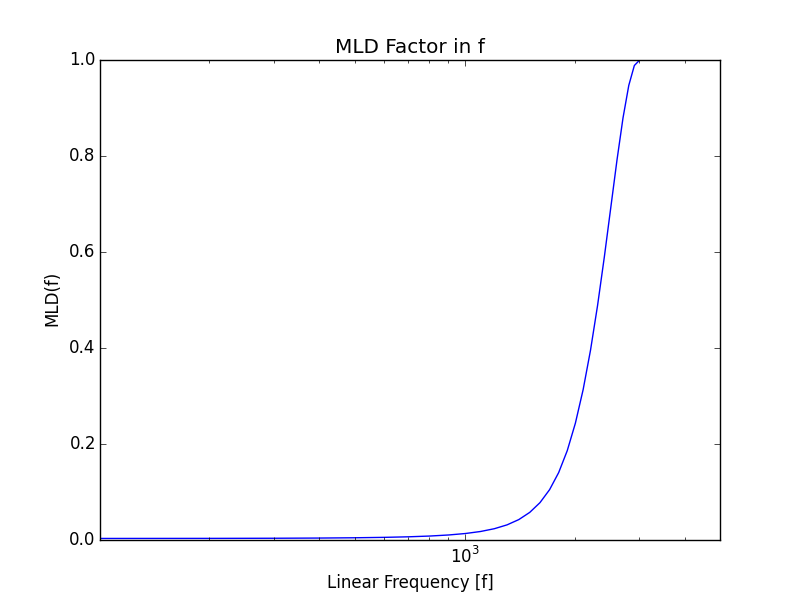
\includegraphics[width=3.5 in]{mld_f_2}
\caption{MLD, Linear Scale}
\label{fig:mldf}
\end{figure}

In this case, where BTHR represents the base threshold (as would be computed for the LR channels) and MLD$_{M,S}$ indicates pointwise multiplication of MLD with BTHR$_{M,S}$ with its masker drops eliminated, the final thresholds for the M and S channels are derived \cite{Johnston1992}.
\begin{align}
\text{THR}_M = \max(\text{BTHR}_M, \min( \text{BTHR}_S, \text{MLD}_S )
\end{align}
\begin{align}
\text{THR}_S = \max(\text{BTHR}_S, \min( \text{BTHR}_M, \text{MLD}_M )
\end{align}

If one imagines a very small S channel masking curve, it is reasonable to find that the M channel could mask signals on the S channel. We had a lot of trouble deciding on the proper way to implement these curves and eventually arrived at a critical understanding of what is required for M/S encoding to meet or exceed the quality of L/R encoding. In actuality, the coding gains that are derived from SMRs reaching an arbitrarily defined threshold in the bit allocation routine must offset the additional bits that are required to meet the lower masking curves that are a result of binaural unmasking.

A second masking threshold that we experimented is detailed below, but we found that the extreme unmasking at low frequencies bit starved other bands, making the curves all but unusable.
\begin{align*}
\text{THR}_M = \min(\text{MLD}_M, \min( \text{BTHR}_M, \text{BTHR}_S )
\end{align*}
\begin{align*}
\text{THR}_S = \min(\text{MLD}_S, \min( \text{BTHR}_M, \text{BTHR}_S )
\end{align*}

Future integration of these more theoretically satisfying threshold calculations with the current, practically determined calculations will be considered below.

\subsection{Bit Allocation and Encoding}
Once the SMRs have been calculated on a band-by-band basis and the LR/MS MDCT lines have been collated into two channels, bit allocation and encoding can proceed in the same manner as regular LR encoding, with only slight changes to the bit allocation routine intended to take advantage of the bit savings as a result of the S-channel's size. By implementing a threshold (dependent on whether or not a channel is MS) on SMRs below which a particular band will no longer accept bits, not every bit in the budget is spent.

Previously, the water-filling algorithm utilized would run until the budget was exhausted; however, if SMRs are arbitrarily low (as they tend to be when allocating S bands), then below a threshold where the quantization noise is inaudible, it doesn't make sense to spend those bits and instead allocate them to blocks with more demanding SMRs.

In the second coder M/S switching algorithm, we keep the SMRs for L, R, M, and S, and run the bit allocation routine with each. Then, by comparing the sum of bits allocated in each band for L and R or M and S, we can pick the allocation scheme that minimizes the number of bits spent. Rather than reducing to two channels during the SMR calculation process, we wait until this point to make the decision, then generate our band encoding flags and the final MDCT lines that will become mantissas.

\subsection{VBR Pool}
As mentioned before, the leftover bits from the truncated bit allocation routine are saved for future blocks in the extraBits coding parameter, which can accrue unused bits until a challenging block (with little masking or wideband noise) appears, at which point the excess can be spent. Because of the lack of look-ahead, the coder never borrows from the future.

Additionally, the Huffman routine returns saved bits to the reservoir, enabling the coder to use these bits to improve the quality in challenging blocks as well.

Generally speaking, although a variable data rate has a net positive effect, it can be a problem for transmission or decode-on-playback applications, especially when considering the more complex allocation schemes that have the possibility of overborrowing.

\subsection{Reconstruction}
Naturally, one must reconstruct the original MDCT from the LR and MS mantissas in much the same way they were encoded in the first place. Rearranging the equations given above result in the following (lossless) reconstruction equations (which work in the time and frequency domains)\cite{Bosi2002}.
\begin{align*}
L_i &= M_i + S_i
\end{align*}
\begin{align*}
R_i &= M_i - S_i 
\end{align*}

Stepping through the decoded MDCT lines on a band-by-band basis, the LR MDCT can be recreated before the regular windowing, IMDCT, and overlap-and-add operations that complete the reconstruction of the signal.

\subsection{Results}
Printed below are the masking thresholds, MDCTs, and SMRs for a particular block in the SQAM German Male Speech test track. Notice in particular the raised masking threshold in the S channel (where the Actual Threshold rises above the Basic Threshold in MDCT lines 100$\sim$600) which arises as a result of the modified threshold selection code detailed above.

% LR FIGURE
\begin{figure}[ht] 
\centering
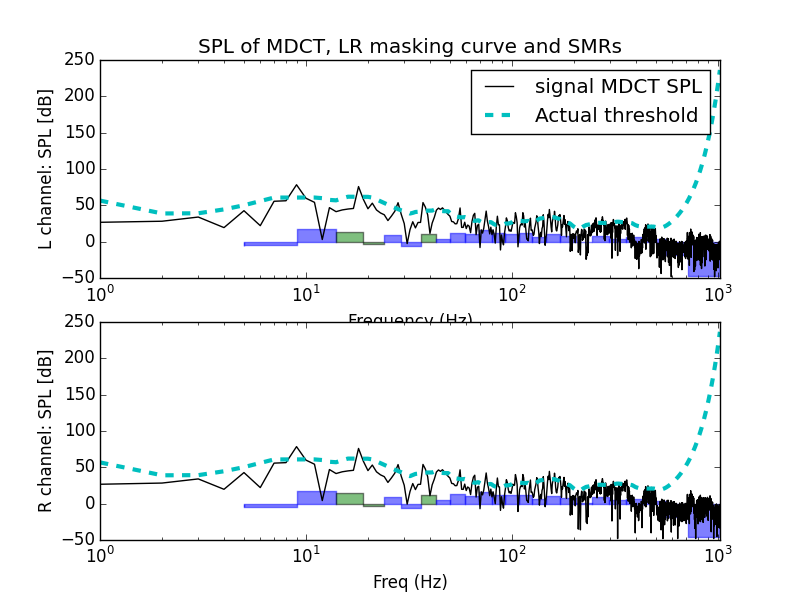
\includegraphics[width=3.5 in]{LR_Threshold}
\caption{Left and Right Channels}
\label{fig:LRTHR}
\end{figure}

% MS FIGURE
\begin{figure}[ht] 
\centering
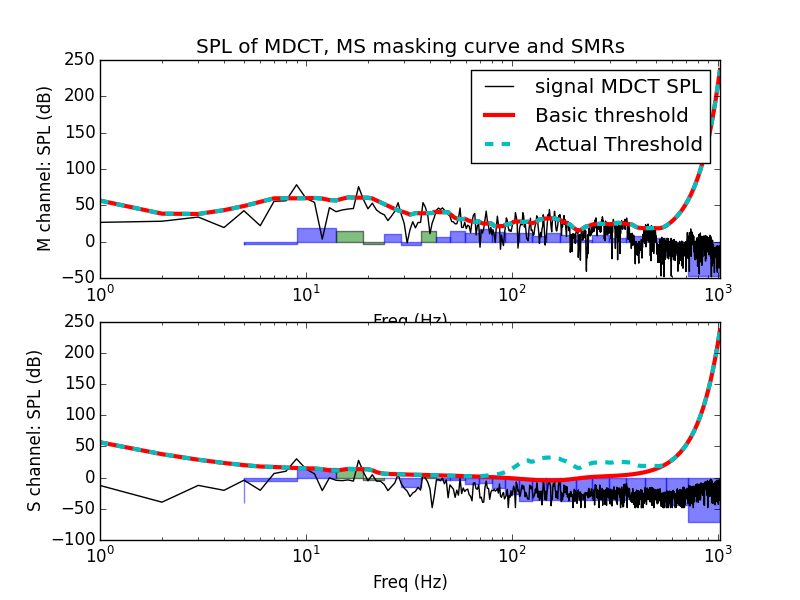
\includegraphics[width=3.5 in]{MS_Threshold}
\caption{Middle and Side Channels}
\label{fig:MSTHR}
\end{figure}

In these plots, a green SMR (indicated by the bar plot) means that LR encoding was selected for that block. Conversely, if the bar is purple, then MS encoding was selected as a result of an increased coding gain that corresponds with a sum of SMRs lower than that of its LR critical band counterpart. 

Generally speaking, with only M/S encoding (not Huffman), we see higher compression ratios, except in audio files that are highly decorrelated, where the compression ratio is similar but depending on the LR / MS selection algorithm that is used, different coding artifacts become apparent. For audio files that are dual mono, massive coding gains and transparent reproduction are present as expected. We found that harmonic signals were difficult to deal with, resulting in birdies for both SQAM harpsichord and trumpet, but as always, these issues could likely be dealt with through improved masking thresholds and LR / MS selection.

\section{Takeaways}
Generally speaking, the increased complexity of Huffman and stereo coding obfuscated the true crux of the coding algorithm that centers on the balance between coding gain and coding quality. Despite all of the improvements that were made, the lack of trustworthy (or even consistent) information about stereo coding in the literature coupled with the abject failure of some theoretically infallible algorithms means that to form a reliable stereo coder, precise definitions of the exact logic for binaural masking thresholds must be defined. 

\subsection{Huffman Coding}
In static Huffman coding, there are two major factors determining the performance of results. One is the way static Huffman coding addresses undiscovered symbols during the training stage, and the other is the static tables pre-constructed prior to encoding general audio files. It would be helpful if there were more literature on different ways of training the static Huffman tables and also how many samples are required to give a desired performance. Due to the time constraint of this project, we could only explore a limited number of training tables. Using more sample audio files to provide a more reliable static Huffman table list would definitely be a rewarding direction to explore provided a longer project duration.

\subsection{Stereo Coding}
Despite our codec not achieving full quality given a particular M/S switching case, it is clear that more structure and modularity is necessary to ensure that the best decision is being made regardless of source material. Forcing our coder into only coding LR (without Huffman) is the same as running the baseline, which is the best decision for highly decorrelated signals; however, some combination of the masking curve selection, bit allocation thresholds, and the power-per-band selection algorithm often select an nonoptimal combination that results in bit starvation and decreased quality that need to be addressed.

% ensure same length columns on last page (might need two subsequent latex runs)
\balance

\section{Future Work}
Regardless of LR or MS, dynamic thresholds for the bit allocation routine could be computed based off of block-to-block changes in SMR levels, channel correlation, and other perceptual factors in order to optimally decide where bit savings should take effect.

A more robust system for deciding between LR and MS could be considered in order to optimize the speed of the coder and the tradeoff between quality and coding gain with a more tunable ability to select stricter reproduction (to rely more upon the baseline LR encoding).

The psychoacoustic model that is currently in use seems logically incoherent with what the literature explains to be the case. Further research and experimentation to determine the legitimate masking curve decision parameters would be extremely beneficial, if only to simplify tuning other parameters that affect the fine balance between coding gain and quality.

A more sophisticated system for integrating the Huffman coding VBR pool to work with stereo coding is also needed. Since the audio quality depends on the bit starvation of each block, we must provide a more efficient way of reallocating bits only to the blocks that can enhance audio quality more significantly instead of consistently giving bits savings away at each block. 

There are certainly other parameters to explore in Huffman coding provided sufficient time. For instance, experimenting with the threshold used for grouping infrequent symbols, constructing escape codes, and also pre-constructing a more diverse static Huffman table distribution in the training stage have high potential for improving compression ratios.    

% MLD-Z FIGURE
\begin{figure}[ht] 
\centering
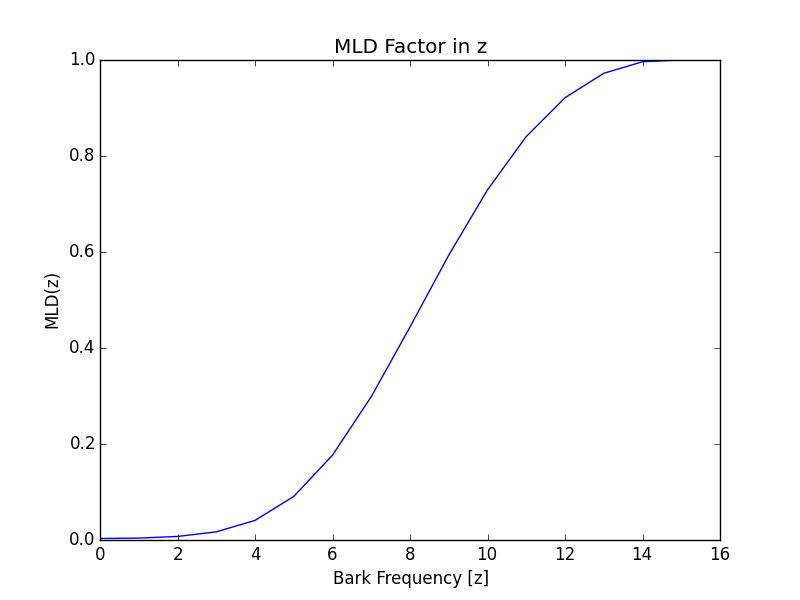
\includegraphics[width=3.5 in]{mld_z}
\caption{MLD, Bark Scale}
\label{fig:mldz}
\end{figure}

%\end{document}

\bibliographystyle{abbrv}
\bibliography{references}

\end{document}